% !TEX root = DesignDocument.tex


\chapter{Project Management}
This section provides some housekeeping type of information with regard to the 
team, project, environment, etc. 



\section{Team Member's Roles}
%Describe who was involved and what role(s) were played. 

Product development is divided into two teams:
\begin{enumerate}
    \item Web Team:
        \begin{itemize}
            \item Daniel Hodgin
            \item Brady Shimp (Scrum Master)
            \item Savoy Schuler
        \end{itemize}
    \item Conversion Software Team:
        \begin{itemize}
            \item Aaron Alphonses
            \item Cheldon Coughlen (Team Lead)
            \item Kenneth Petry
        \end{itemize}
\end{enumerate}

The website team shares the responsible for developing the website, file upload and download abilities, an API for connecting the website to the conversion software, user log in protected profile functionality, user abilities to manage files, social/collaborative features, file permissions and cloud hosting abilities.  


The conversion software shares the responsible for developing software to convert uploaded file types into file types render-able by AR devices and applications needed by devices for reading and rendering files from QR codes.


As Team Lead, Cheldon Coughlen acts as the team representative to the sponsor and client and brokers communication between these parties and the development team. 

As Scrum Master, Brady Shimp manages the task board and delegates tasks. 

\section{Project  Management Approach}
This section will provide an explanation of the basic approach to managing the 
project.  Typically, this would detail how the project will be managed through 
a given Agile methodology.  The sprint length (i.e. 2 weeks) and product backlog 
ownership and location (ex. Trello) are examples of what will be discussed.  An 
overview of the system used to track sprint tasks, bug or trouble tickets, and 
user stories would be warranted. 

The product is being approached with Agile methodology and two week sprints. InTouch L.L.C. COO Brady Shimp owns the backlog which is located on the GitHub project repository. Mr. Shimp creates tickets which are placed in the backlog. Developers will select tickets, attach their name to it, and move it to an "In Progress" bin to denote activity. Tickets may be assigned by Mr. Shimp or selected by unoccupied developers. Priority levels are assigned to tasks, bugs, and user stories to indicate the priority of the respective ticket. These priority levels may be assessed by whether the ticket roadblocks other development, necessity of the feature based on milestones, or urgency otherwise established.

\section{ Stakeholder Information}


% This section would provide the basic description of all of the stakeholders for 
% the project. Who has an interest in the successful and/or unsuccessful completion of this project? 

\begin{itemize}
	\item InTouch L.L.C.: Custom software solutions company needs product to fulfill contractual obligations to client. 
	\item South Dakota School of Mines and Technology: Higher education STEM university needs investment in product to result in development of circular material and provide application in classrooms.
\end{itemize}


\subsection{Customer or End User (Product Owner)}
% Who?  What role will they play in the project?  Will this person or group manage 
% and prioritize the product backlog?  Who will they interact with on the team to 
% drive product backlog priorities if not done directly? 

The direct customer is the South Dakota School of Mines and Technology with faculty members such as Dr. Jeff McGough, Dr. Christer Karlsson. Dr. Adam Piper, Dr. Brent Deschamp, and Dr. King Adkins constituting an initial base of end users. These faculty members are directly involved with the creative direction of the product and are the indirect source of the product backlog. The faculty members meet monthly with the development team to develop user stories. Two faculty members, Dr. Jeff McGough and Dr. Christer Karlsson, meet weekly with the development team to provide direct input on the backlog and direction of the product. 

\subsection{Management or Instructor (Scrum Master)}
% Who?  What role will they play in the project?  Will the Scrum Master drive the 
% Sprint Meetings? 

Brady Shimp, COO of InTouch L.L.C., is the Scrum Master of this project. Brady developed the project time-lines and milestones and actively manages the task board and drives delegation. Brady leads sprint meetings and stand-ups. 


\subsection{Investors}
%Are there any?  Who?  What role will they play? 

No investors are involved with the Sponsor or its product. 

\subsection{Developers --Testers}
% Who?  Is there a defined project manager, developer, tester, designer, architect, 
% etc.? 

Developers are assigned components of the platform on constant rotation. Each developer is required to play all roles regarding their component. This includes, but is not limited to, designing, architecting, managing, developing, and testing their solution. In the designing and architecting phase, a developer is required to consult the members of their development team to ensure proper planning and compatibility. Each developer must have their functioning implementation thoroughly verified by another team member before merging their solution into the development branch. 

As a whole, the project development and testing is managed by Brady Shimp. Mr. Shimp manages the development of the project through the task board by creating, delegating, and monitoring the completion of tickets. 

\section{Budget}
% Describe the budget for the project including gifted equipment and salaries for 
% people on the project.

There is no budget actively established for the project. Pending official adoption of the product by the South Dakota School of Mines and Technology, proper withholdings will be made to support a year of operation of the product. All other profit will be allocated evenly among the student development team. 

\section{Intellectual Property and Licensing}
% Describe the IP ownership and issues surrounding IP.

All intellectual property and ownership is retained by InTouch L.L.C.. 

Licenses for Visual Studio 2017 need not be purchased as students are already granted licensed access. All other third party resources utilized are available under the MIT License or likewise. 


\section{Sprint  Overview}
The development cycle that is being followed is a feature driven development.
The features and milestones created at the beginning of the semester.
Sprint were handled in two week incriments and features were assigned to 
the sprints to be accomplished during the two weeks. The backlog consisted
of what was going to be accomplished in the coming weeks and what was not
completed in the last sprint. At the begining/end of each sprint, the 
developers would get together for a sprint retrospective, to discuss
how to previous sprint went and how to handle the up coming one.


\section{Terminology and Acronyms}
% Provide a list of terms used in the document that warrant definition.  Consider 
% industry or domain specific terms and acronyms as well as system specific. 

\begin{itemize}
	\item Augmented Reality (AR): hardware and software that, together, superimpose computer-generated images on a user's view of the real world. Often, this composite view may be interacted with. 

	\item Virtual Reality (VR): hardware and software that, together, create a computer-generated simulation of a three-dimensional image or environment. Often, this simulation may be interacted with. 

	\item Mixed Reality (MR): the overlap in domain space of augmented reality and virtual reality. 

	\item Microsoft HoloLens: portable and cordless augmented reality viewing device. 

	\item Meta Meta 2: augmented reality viewing device that must be connected to a computer and power outlet. 

	\item Mira Prism: augmented reality viewing device that leverages a user's mobile device.

	\item Oculus Rift: virtual reality viewing device. 

    \item QR Code: machine readable matrix barcode optical label.
    
    \item Unity: video game engine used in creating HoloLens apps.

	\item Cloud: off-site computing and digital storage resources accessed via the internet. 

    \item Azure: Microsoft Cloud hosting feature

	\item .fbx: model file type that may be rendered by most AR devices on the market. 
\end{itemize}


\section{Sprint Schedule}
As stated above, sprints were two weeks long. Each sprint was designed to accomplish a milestone. 
Below is the schedule of the sprints and what was accomplished during those sprints.

\begin{itemize}
	\item 9/18/2017    - Define milestones and user stories
	
	\item 10/2/2017    - Base website created with file upload

	\item 10/16/2017  - Wireframes, Presentation 1 Documents, Standalone file conversion

	\item 10/30/2017  - File Upload/Download, File Conversion Integrated

	\item 11/13/2017  - QR code generation, Standalone advanced file conversion 

	\item 11/27/2017 - File Conversion Integration, Create users, Presentation 2 Documents

	\item 12/4/2017   - Finish Documentation, Next semester prep


	
\end{itemize}

\section{Timeline}
Below is the timeline of accomplished milestones.

\begin{figure}[H]
\begin{center}
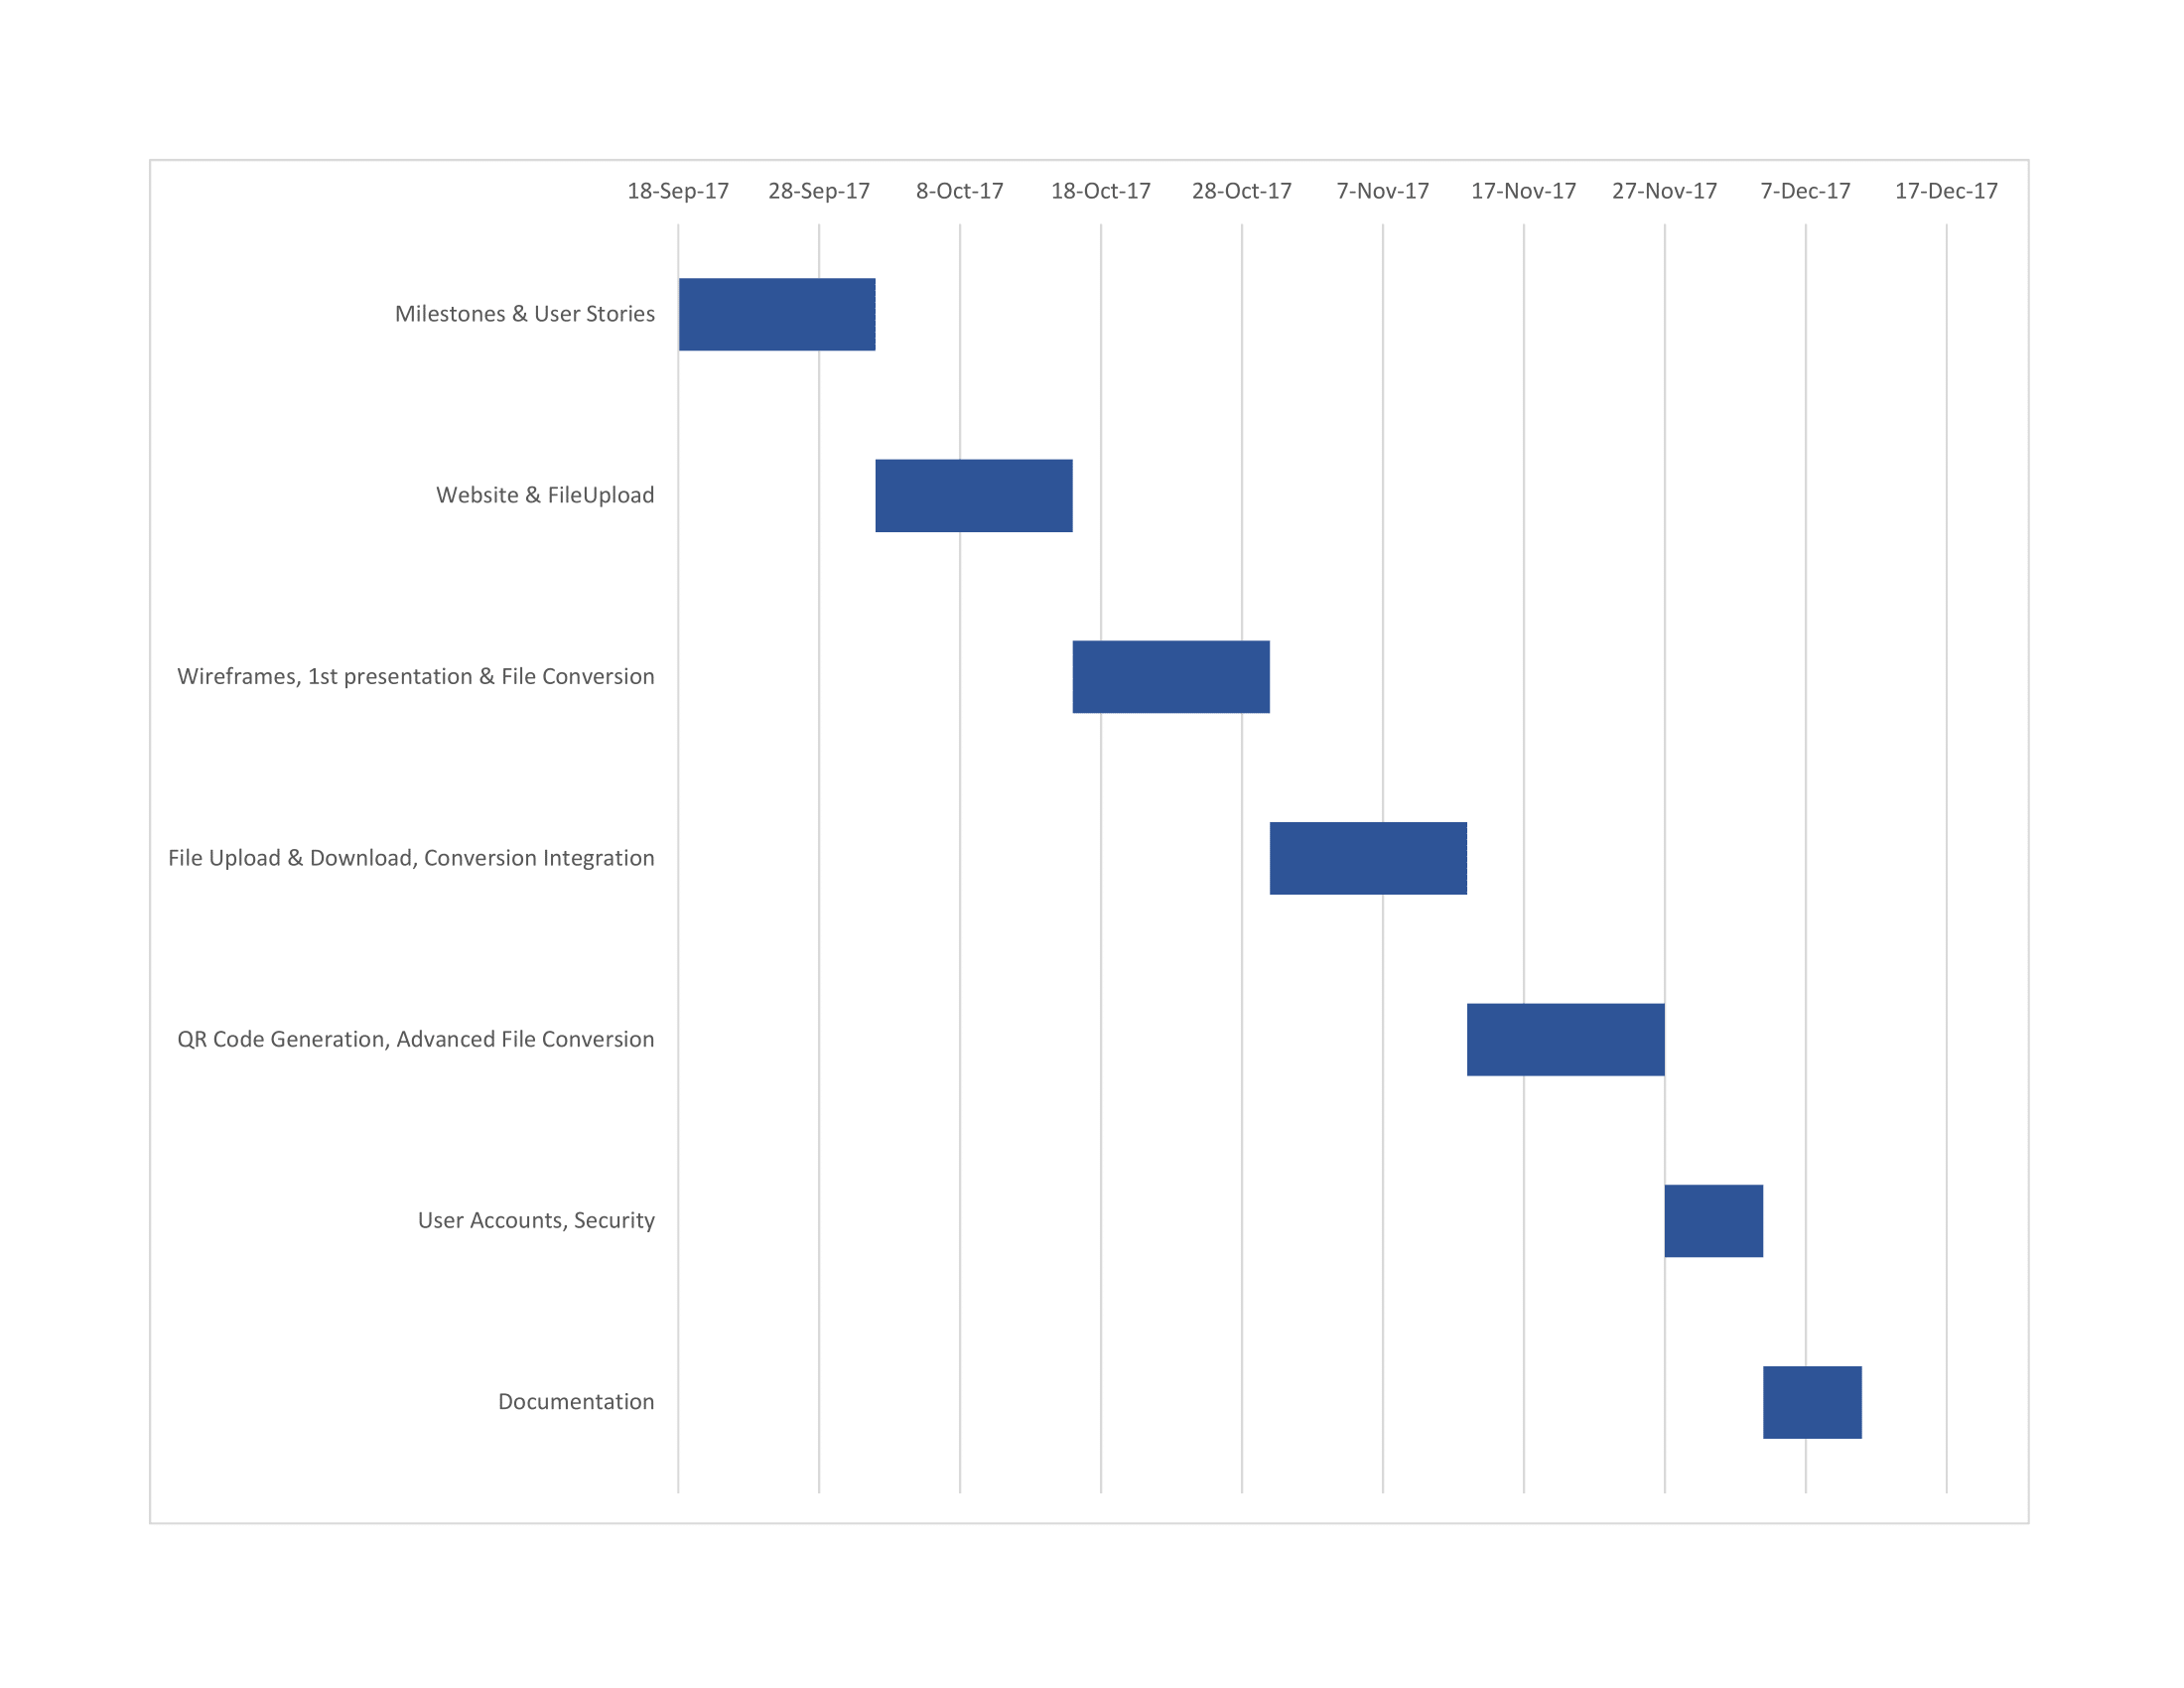
\includegraphics[width=1\textwidth]{./SprintGanattChart}
\end{center}
\caption{Sprint Timeline}
\end{figure}

\section{Development Environment}
%The basic purpose for this section is to give a developer all of the necessary 
%information to setup their development environment to run, test, and/or develop. 
The Microsoft enviroment was choosen for the simplicity of the Azure Cloud hosting tools and 
the store ties the product has to Microsoft's Hololens. Specifically, ASP.net MVC is being used in creation of the website.
SQL server was chosen, also for it simplicity in integratign with Azure.

\section{Development IDE and Tools}
%Describe which IDE and provide links to installs and/or reference material. 

The IDE of choice for the website and file conversion team is Visual Studio 2017 Enterprise Edition.
Microsoft SQL Server Management Studio is used for the database.
Unity Game Engine is used for Hololens App Dvelopment

\paragraph{}
The tools needed for website development are.
\begin{itemize}
    \item ASP.NET framework
    
    \item Azure Cloud Hosting Tools

    \item Both tools can be aquired from the Visual Studio Installer

\end{itemize}

\paragraph{}
To compile the web conversion software two libraries are needed.
\begin{itemize}
    \item Autodesk's FBX SDK is required to export .fbx files.  It must be installed in a folder located in the project directory nmed \"FBX SDK\".  The download can be found at: 
    \url{http://usa.autodesk.com/adsk/servlet/pc/item?siteID=123112&id=26416244}.
    The Windows VS2015 version must be installed.
    
    \item Open Asset Import Library supports a wide variety of import and export file types.  The download can be found at: \url{http://assimp.org/main_downloads.html}.  Version 3.1.1 is what was used in the project. 
\end{itemize}

\paragraph{}
To develop the Hololens application, the following tools are needed:
\begin{itemize}
    \item Unity Personal: Unitiy game engine editor that is free for company use, if you make lower than 100,00 dollars per year. 
    \item Visual Studio Tools for Unity - Can be downloaded from Visual Studio installer.
    \item HoloToolkit-Unity Set of tools for Hololens development with unity. Free for use. Download from the GitHub page.
\end{itemize}


\section{Source  Control}
Github was used to manage the source code. It was picked, because it was most well known amongst the
developers. It was set up wth the with three branches, Master, Develop and Release. The work is done on the Develop branch
and once it is throughly tested it is then pushed up to release.

The following steps were taken to contribute to the code.
	
I am trying to make this into a list and it is giving me an hbox overfull and justifying the text to the right in the pdf. I simply want to put numbers on this and make a list.

\begin{enumerate}

\item Pull latest code from the develop branch
\item Impliment feature
\item Push to Develop and assign other developer for QA
\item Once properly tested, push to Release branch.

\end{enumerate}

\section{Dependencies}
%Describe all dependencies associated with developing the system. 
\paragraph{Website}
\begin{description}
    \item ASP.NET MVC Framework is used for front and backend.
\end{description}

\paragraph{File Conversion}
\begin{description}
    \item [FBX SDK] A library produced by Autodesk that converts from a select few file types to the .fbx file that is easily viewed on Microsoft supported software (Windows 10, Hololens).
    \item [Open Asset Import Library] A library the reads and writes multiple file types (does not export to .fbx).
\end{description}

\section{Build  Environment}
Azure is used to build and deploy the website. Once the tools are downloaded and an Azure account is created, 
all that is needed is to right-click on the ASP.NET MVC project and select publish. The website is then hosted on Azure and
can be accessed by all.
\section{Development Machine Setup}

Pull the git repository with both the Website and File Conversion code located at: \url{https://github.com/SavoySchuler/ARFE}

% If warranted, provide a list of steps and details associated with setting up a 
% machine for use by a developer. 

The following are the requirement for a development machine:
\begin{itemize}
    \item Windows 10
    \item Visual Studio 2017 Enterprise with ASP.NET MVC, Azure and Unity tools
    \item Unity Personal
    \item HoloToolkit-Unity Set of tools for Hololens development with unity. Free for use. Download from the GitHub page.
\end{itemize}

\paragraph{File Conversion}

There are two libraries that need to be installed: Assimp and FBX SDK.

\subparagraph{FBX SDK}

\begin{enumerate}
    \item Got to the following link and install the FBX SDK.
    \begin{itemize}
        \item \url{http://usa.autodesk.com/adsk/servlet/pc/item?siteID=123112&id=26416244}
        \item Use the installer under: Windows / FBX SDK 2018.0 VS2015
    \end{itemize}

    \item Copy the FBX SDK folder to the directory with the source code (the deepest FileConverion folder)
    \begin{itemize}
        \item At the location of the installiation, the file structure should be: Autodesk/FBX/FBX SDK/
        \item Copy the FBX SDK folder to the source code directory.
    \end{itemize}
\end{enumerate}

\subparagraph{Assimp}

\begin{enumerate}
    \item Go to the following link and install the Assimp software.
    \begin{itemize}
        \item \url{http://assimp.org/main_downloads.html}
        \item Version 3.1.1 is what was used during development.
    \end{itemize}

    \item From the installiation location, copy the \"Assimp\" folder into the deeper FileConverion directory.
    \begin{itemize}
        \item Paste the folder into the same folder as the source code of the File Conversion.
    \end{itemize}

    \item Copy FileConverion/Assimp/bin/x86/assimp-vc140-mt.dll to the same directory as the source code.
\end{enumerate}